\documentclass[../main.tex]{subfiles}

\graphicspath{{../figures}}

\begin{document}

\mychapter{理论基础与预备知识}\label{sec:ch2-theoretical-foundations}

本章旨在为后续章节深入探讨深度模型高效构建的具体方法奠定必要的理论基础。我们将集中阐述贯穿本文研究的核心理念,界定关键问题领域的形式化定义,并统一全文所使用的数学符号。通过提供这些预备知识,本章力求为读者理解后续提出的 Prompt-Distiller(第 \ref{sec:ch3-dual-contrastive-distillation-for-few-shot-prompts} 章)、\textsc{Bridge}(第 \ref{sec:ch4-evolutionary-transfer-nas-heterogeneous-spaces} 章)与 KG-MFTO(第 \ref{sec:ch5-knowledge-guided-multi-form-optimization-for-llm-fusion} 章)等创新性方法扫清障碍,确保论述的严谨性与一致性。

\mysection{引言}
\label{sec:ch2-1-introduction}

如第一章所述,本文的核心目标是探索基于知识迁移思想的深度模型高效构建方法,并分别在知识、结构与参数三个关键维度上展开独立研究。为了清晰、严谨地阐述这些研究工作,有必要首先建立一个共同的理论基础和术语体系。本章(第二章)正是承担了这一关键的奠基任务。

具体而言,本章将首先在 \ref{sec:ch2-2-knowledge-transfer-core-ideas} 节深入界定知识迁移这一核心视角在本文语境下的具体内涵,并阐明其在知识、结构、参数三个层面上的不同表现形式与知识载体。随后,\ref{sec:ch2-3-formalizing-key-problem-domain} 节将对后续章节重点关注的三个关键问题领域——即少样本学习与知识蒸馏、NAS与可迁移 NAS、以及模型参数融合——给出最核心、最形式化的问题定义,为后续方法的设计提供清晰的问题边界。最后,\ref{sec:ch2-4-chapter-summary} 节将对本章内容进行简要总结。

本章的定位是提供必要且精炼的预备知识。 关于相关工作的历史演进、方法细节、优劣对比及局限性分析,已在第一章 \ref{sec:ch1-2-global-research-status} 节国内外研究现状中完成,或将在后续相应的方法章节中结合具体创新点进行阐述。

\mysection{知识迁移的核心理念与体现}
\label{sec:ch2-2-knowledge-transfer-core-ideas}

知识迁移构成了贯穿本文研究的核心理念与视角。正如第 \ref{sec:ch1-preface} 章所深入剖析,深度学习在取得巨大成功的同时,也日益面临由数据、算力与人力投入急剧增长所带来的规模-效率困境。在此背景下,知识迁移提供了一种旨在通过系统性地复用与传递已有知识资产,以应对资源约束、提升模型构建全流程效率的方法论思想\cite{surveytransferlearning_pan_2010}。其根本出发点在于,认识到在过往的模型训练、架构设计乃至问题求解过程中,有价值的知识已被大量生成并固化于各种载体之中——无论是数据集内蕴含的复杂统计模式,成功网络架构所体现的有效计算原理,还是预训练模型参数中编码的泛化表征\cite{bertpretraining_devlin_2019}。知识迁移的核心理念,正是充分挖掘信息的价值,将这些既有知识视为可复用的资源,通过有效的机制将其迁移至新的任务或模型构建过程中,从而避免代价高昂的从零开始,实现更智能、更经济的深度学习实践。

在本文的研究语境中,知识迁移并非局限于特定的技术分支(如狭义的迁移学习或知识蒸馏),而是指代一种更广义的指导原则:即在模型构建的各个环节,主动地识别、提取并在不同阶段或不同模型间传递有价值的先验信息,用以指导学习、加速收敛、提升性能或降低资源消耗。本文正是基于这一核心理念,分别在深度模型构建的知识、结构与参数三个关键维度上展开独立探索。这三个维度代表了知识在深度学习模型中存在和流动的不同层面,也因此为知识迁移思想的应用提供了不同的切入点和具体体现:

其一,在知识层面,知识迁移主要体现为模型所学习到的抽象语义知识与判别能力的传递。这里的知识通常指模型通过大规模数据训练所获得的、超越具体样本的、具有一定通用性的理解,例如对输入数据(如图像、文本)的层次化特征表示、对不同概念或类别之间关系的捕捉、乃至在特定任务(如推理、生成)中形成的隐式规则或启发式策略。当面临新任务,特别是标注数据稀缺(如少样本学习)的情况时,直接从头学习这些复杂的抽象知识是极其困难的。此时,将一个已在相关或通用大规模数据上训练好的教师模型所掌握的这种抽象知识,通过某种机制(如知识蒸馏)迁移给资源受限下训练的学生模型,便成为提升后者性能与泛化能力的关键途径。知识蒸馏正是实现此类知识传递的代表性技术\cite{modelcompression_bucilua_2006,distillingknowledgeneural_hinton_2015,fitnetshintsthin_romero_2015}。本文第 \ref{sec:ch3-dual-contrastive-distillation-for-few-shot-prompts} 章的研究工作即聚焦于此,旨在探索如何在少样本条件下,设计更鲁棒的蒸馏机制以实现这种语义知识的高效与稳定迁移。

其二,在结构层面,知识迁移则体现为神经网络架构设计模式与搜索优化经验的传递。一个优良的网络架构本身就是一种强大的知识载体,它凝结了关于如何针对特定数据类型(如图像的空间结构、文本的序列依赖)和计算目标(如特征提取、信息融合)进行有效信息处理的结构性知识。例如,在先前任务中被验证有效的架构组件(如 Inception 模块、Transformer 层)\cite{goingdeeperconvolutions_szegedy_2015,attentionisall_vaswani_2017}、连接模式或整体拓扑结构,均可作为可迁移的结构先验。更细化地说,卷积层利用了平移不变性,残差连接促进了梯度传播,自注意力机制捕捉了长距离依赖 \cite{imagenetclassificationdeep_krizhevsky_2012,deepresiduallearning_he_2016,attentionisall_vaswani_2017}。当面临自动化设计新架构(如 NAS)的需求时,如果能够迁移上述被证明有效的组件与策略,就能显著缩小搜索空间、加速最优架构的发现过程。这种结构性知识的迁移是 TNAS 的核心目标 \cite{archgraphacyclic_huang_2022,emtnastransferring_liao_2023}。然而,实现这种迁移,特别是在架构范式存在显著差异(异构搜索空间)的情况下,面临巨大挑战。本文第 \ref{sec:ch4-evolutionary-transfer-nas-heterogeneous-spaces} 章的研究工作正是致力于突破这一瓶颈,探索如何实现结构知识在异构搜索空间之间的有效传递。

其三,在参数层面,知识迁移以一种最为直接的形式体现,即已训练模型参数权重本身的传递、调整与组合。现代深度学习,尤其是基于大规模预训练模型的范式,其核心优势就在于预训练模型参数中已经编码了海量的通用世界知识和语言/视觉基础能力 \cite{bertpretraining_devlin_2019,languagemodelsare_brown_2020}。传统的微调和参数高效微调(如 Adapters、LoRA)本质上就是对这些参数知识进行适配和利用 \cite{parameterefficienttransfer_houlsby_2019,loralowrank_hu_2022}。而模型融合则探索了更进一步的可能性:能否在完全免训练的条件下,通过直接操纵和组合来自不同专长模型的参数,快速构建出具备集成能力的新模型?这一路线已在权重平均与加权融合等方法中得到初步验证 \cite{modelsoupsaveraging_wortsman_2022,mergingmodelsfisher_matena_2022,editingmodelstask_ilharco_2023}。这种方式旨在通过对参数知识的直接迁移与整合来实现能力的即时构建。然而,如何智能地进行参数组合以避免冲突并保留各自优势,是其核心难题 \cite{gitrebasin_ainsworth_2023,losssurfacesmode_garipov_2018}。本文第 \ref{sec:ch5-knowledge-guided-multi-form-optimization-for-llm-fusion} 章的研究工作将聚焦于此,研究如何通过知识引导的优化策略,实现这种参数知识的高效、稳定融合。

综上所述,知识迁移作为本文的核心指导理念,其内涵与实现在不同层面各有侧重:知识层关注抽象语义知识的迁移,依赖于模型间的映射与对齐;结构层关注设计模式与经验的迁移,依赖于架构的表示与演化;而参数层则关注具体参数权重的迁移与组合,依赖于对参数空间几何与知识兼容性的理解。正是基于对知识迁移在不同维度上多样化体现及其面临挑战的认识,本文分别展开了后续三个章节的独立研究。这些研究虽各有侧重,但共同构成了对“基于知识迁移的深度模型高效构建”这一核心命题的多方位探索与回应。

\mysection{关键问题领域形式化定义}
\label{sec:ch2-3-formalizing-key-problem-domain}

在明确了知识迁移作为贯穿本文研究的核心视角后(2.2 节),本节将进一步对本文重点关注的三个关键问题领域进行形式化的界定。清晰的问题定义是展开严谨研究的前提。我们将分别对少样本学习(Few-Shot Learning, FSL)与知识蒸馏(Knowledge Distillation, KD)、神经架构搜索(Neural Architecture Search, NAS)、以及免训练模型融合这三个领域的核心问题进行数学化描述,旨在为后续章节(第三、四、五章)中提出的具体方法提供精确的问题背景与优化目标。

\mysubsection{小样本学习与知识蒸馏}
\label{sec:ch2-3-1-few-shot-learning-and-distillation}

\textbf{小样本学习(Few-Shot Learning, FSL)} 研究的核心在于,当模型面临全新的类别且每个类别仅能提供极少数标注样本时,如何快速学习并具备对这些新类别样本的识别或处理能力。在监督学习,特别是分类任务的背景下,FSL 通常被构建为一系列的 \textbf{N-way K-shot} 情节或任务 $\mathcal{T}$。每个任务 $\mathcal{T}$ 包含一个支持集$\mathcal{S} = \{(x_i^s, y_i^s)\}_{i=1}^{N \times K}$ 和一个查询集$\mathcal{Q} = \{(x_j^q, y_j^q)\}$。支持集 $\mathcal{S}$ 提供了 $N$ 个不同类别的信息,且每个类别恰好包含 $K$ 个标注样本(其中 $K$ 是一个很小的整数,如 1, 5, 或 16)。查询集 $\mathcal{Q}$ 则包含来自相同 $N$ 个类别、但与支持集样本不同的新样本,用于评估模型在该任务上的泛化性能。FSL 的目标是学习一个模型 $f_\theta$(或者一个学习算法),使其能够利用给定任务 $\mathcal{T}$ 的支持集 $\mathcal{S}$,对该任务的查询集 $\mathcal{Q}$ 做出准确的预测。形式上,这通常被表述为最小化在任务分布 $p(\mathcal{T})$ 上的期望损失:
\begin{equation}
	\min_\theta \mathbb{E}_{\mathcal{T} \sim p(\mathcal{T})} \left[ \mathcal{L}\left(f_\theta(\mathcal{Q}|\mathcal{S}), \mathcal{Y}^q\right) \right]
	\label{eq:fsl_objective}
\end{equation}
在此优化目标中,$\theta$ 代表模型 $f$ 的可学习参数,$\mathbb{E}_{\mathcal{T} \sim p(\mathcal{T})}$ 表示在任务分布 $p(\mathcal{T})$ 上取期望,意在寻求在各种可能的少样本任务上的平均最优性能。$f_\theta(\mathcal{Q}|\mathcal{S})$ 表示模型利用支持集 $\mathcal{S}$ 提供的信息对查询集 $\mathcal{Q}$ 做出的预测结果,$\mathcal{Y}^q$ 则是查询集 $\mathcal{Q}$ 对应的真实标签集合。$\mathcal{L}$ 为适用于具体任务的损失函数,例如分类任务中常用的交叉熵损失。FSL 的根本挑战在于如何从极度有限的类别内信息 $K$ 中学习到具有泛化能力的类别表示或判别边界\cite{matchingnetworksone_vinyals_2016,prototypicalnetworksfew_snell_2017,modelagnosticmeta_finn_2017}。

\textbf{知识蒸馏(Knowledge Distillation, KD)} 则提供了一种在模型间传递知识的通用框架。其基本设定涉及一个预训练好的、性能较优的大型教师模型(Teacher Model)和一个待训练的、参数量较小的学生模型(Student Model)。为与后续章节(特别是第三章)保持符号一致性,我们将教师和学生的模型参数分别记为 $\Theta_T$ 和 $\Theta_S$。在某些情况下,我们可能还会利用教师模型在特定任务微调前的原始预训练状态,其参数记为 $\Theta_{T'}$。KD 的目标是训练学生模型 $\Theta_S$,使其能够模仿教师模型(如 $\Theta_T$ 或 $\Theta_{T'}$)的行为。令 $s_{\Theta_S}(x_i)$ 和 $s_{\Theta_T}(x_i)$ 分别表示学生和教师模型在输入 $x_i$ 上的 Logits 输出(或对应的评分函数),标准的蒸馏损失 $\mathcal{L}_\mathrm{KD}$ 通常基于两者经过温度 $T$ 平滑后的 Softmax 概率分布 $p_S$ 和 $p_T$ 之间的 KL 散度来定义:
\begin{gather}
	p_S = \text{Softmax}(s_{\Theta_S}(x_i)/T), \quad p_T = \text{Softmax}(s_{\Theta_T}(x_i)/T) \label{eq:kd_softmax} \\
	\mathcal{L}_\mathrm{KD}(p_T, p_S) = T^2 \cdot D_\mathrm{KL}(p_T || p_S) \label{eq:kd_loss}
\end{gather}
这里,$T > 1$ 是温度系数,用于增大 Logits 除以 $T$ 后的数值差异,从而产生更平滑的概率分布 $p_S$ 和 $p_T$,即学生和教师模型输出的软概率分布。$D_\mathrm{KL}(p_T || p_S)$ 表示教师软分布 $p_T$ 与学生软分布 $p_S$ 之间的 Kullback-Leibler 散度,衡量两者之间的差异。因子 $T^2$ 是一个常用的缩放系数,用于在温度 $T$ 较高时保持蒸馏损失梯度的大致量级,使其与使用硬标签的监督损失梯度相当。学生模型的总训练目标 $\mathcal{L}_{total}$ 通常会结合标准的监督损失 $\mathcal{L}_\mathrm{supervised}$(例如,在第 \ref{sec:ch3-dual-contrastive-distillation-for-few-shot-prompts} 章中将使用基于掩码语言模型预测的损失 $\mathcal{L}_\mathrm{MLM}(X)$~\cite{bertpretraining_devlin_2019})与一项或多项蒸馏损失 $\mathcal{L}_{\mathrm{KD}, j}$(后续章节将引入 $\mathcal{L}_\mathrm{KD}(X), \mathcal{L}_\mathrm{KD}(\tilde{X})$ 等具体形式),并通过权重系数 $\lambda_j$(如第 \ref{sec:ch3-dual-contrastive-distillation-for-few-shot-prompts} 章的 $\lambda_1, \lambda_2$)进行平衡:
\begin{equation}
	\mathcal{L}_\mathrm{total} = \mathcal{L}_\mathrm{supervised} + \sum_j \lambda_j \mathcal{L}_{\mathrm{KD}, j}
	\label{eq:kd_total_loss}
\end{equation}
在此式中,$\mathcal{L}_\mathrm{supervised}$ 代表标准的监督学习损失项(如交叉熵 $\mathcal{L}_\mathrm{CE}$),$\mathcal{L}_{\mathrm{KD}, j}$ 代表第 $j$ 项具体的蒸馏损失,而 $\lambda_j \ge 0$ 则是用于权衡各项损失贡献的系数。通过最小化总损失 $\mathcal{L}_\mathrm{total}$,学生模型被期望在保持对真实标签预测能力的同时,学习到教师模型所传递的更丰富的泛化知识\cite{distillingknowledgeneural_hinton_2015,patientknowledgedistillation_sun_2019}。
本文第 \ref{sec:ch3-dual-contrastive-distillation-for-few-shot-prompts} 章的研究工作将聚焦于上述 FSL 与 KD 两个问题的交叉点所带来的独特挑战。具体而言,研究将在严格的 N-way K-shot 少样本设定下展开,此时核心标注集 $X$ 即为可用的主要监督来源。标准的 KD 框架通常假设存在充足数据。当数据骤减至少样本级别时,如何设计有效的知识传递机制(例如,第 \ref{sec:ch3-dual-contrastive-distillation-for-few-shot-prompts} 章将引入利用无标注数据 $\tilde{X}$ 和对比损失 $\mathcal{L}_\mathrm{CPD}$ 的策略)以克服挑战,便构成了该交叉领域的核心研究问题。

\mysubsection{神经架构搜索}
\label{sec:ch2-3-2-neural-architecture-search}

\textbf{神经架构搜索(Neural Architecture Search, NAS)} 代表了自动化机器学习领域的一个重要研究方向,旨在将原先高度依赖人工经验和大量试错的神经网络架构设计过程自动化。其核心目标是在一个预定义的、通常极其庞大的候选架构集合,即搜索空间 $\mathcal{A}$ 中,通过特定的算法自动地寻找能够针对目标任务和给定数据集达到最优或近优性能的架构 $a^*$。一个架构 $a \in \mathcal{A}$ 严谨地定义了网络的计算图结构,包括其层级组成、节点(通常代表特征图)之间的连接关系、以及在节点或边上执行的具体数学运算(例如卷积层、池化层、自注意力模块等)及其相关配置。搜索空间 $\mathcal{A}$ 本身的设计至关重要,它界定了架构设计的语法规则和基础构件,其表达能力与规模直接影响了最终可能发现架构的性能上限与搜索的难度。例如,搜索空间可以是基于重复单元的微观结构设计,也可以是面向整个网络宏观拓扑的全局规划\cite{neuralarchitecturesearch_elsken_2019}。

从形式化的角度看,NAS 过程通常可以被抽象为一个具有挑战性的双层优化问题:
\begin{align}
	a^{*}                      & = \arg\min_{a \in \mathcal{A}} \mathcal{L}_\mathrm{val}(w^{*}(a), a) \label{eq:nas_outer} \\
	\text{s.t.} \quad w^{*}(a) & = \arg\min_{w \in \mathcal{W}_a} \mathcal{L}_\mathrm{train}(w, a) \label{eq:nas_inner}
\end{align}
在此 \eqref{eq:nas_outer} 和 \eqref{eq:nas_inner} 中,$a$ 代表从庞大的搜索空间 $\mathcal{A}$ 中采样或构建出的一个具体候选神经网络架构。内层优化问题 \eqref{eq:nas_inner} 描述了对给定架构 $a$ 的标准模型训练过程:即寻找一组最优的权重参数 $w^{*}(a)$,使得该架构在训练数据集上的损失 $\mathcal{L}_\mathrm{train}(w, a)$ 最小化。这里,$w$ 表示架构 $a$ 的所有可训练权重,$\mathcal{W}_a$ 是其对应的权重参数空间。外层优化问题 \eqref{eq:nas_outer} 则是在架构空间 $\mathcal{A}$ 中进行搜索:其目标是找到一个架构 $a^*$,当该架构使用其最优权重 $w^*(a)$ 时,在独立的验证数据集上能够取得最低的验证损失 $\mathcal{L}_\mathrm{val}(w^{*}(a), a)$(或其他性能指标)。这个双层结构清晰地揭示了 NAS 的核心困难:外层优化的每一步(评估一个架构 $a$)都需要完整地求解一次内层优化(训练模型 $a$),这使得整个过程计算量极大\cite{dartsdifferentiablearchitecture_liu_2019}。

\begin{figure}
	\centering
	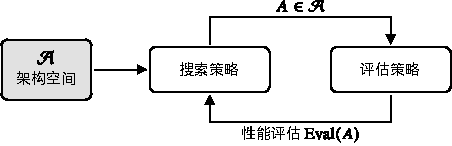
\includegraphics[width=0.67\textwidth]{nas-bilevel.pdf}
	\bicaption[典型NAS框架示意图]{典型神经架构搜索(NAS)框架示意图。NAS 过程通常由搜索空间、搜索策略与性能评估策略三大关键组件协同工作。}[Typical NAS framework]{Illustration of a typical neural architecture search (NAS) framework. The NAS process is usually driven by the coordinated work of the search space, search strategy, and performance evaluation strategy.}
	\label{fig:nas-bilevel-optimization}
\end{figure}

如图 \ref{fig:nas-bilevel-optimization} 所示,典型的 NAS 框架通常由三个关键组件协同工作:首先是定义候选架构集合及其编码方式的\textbf{搜索空间} $\mathcal{A}$;其次是决定如何在 $\mathcal{A}$ 中高效探索、生成新架构的\textbf{搜索策略},例如基于强化学习、进化算法、梯度优化或随机搜索等不同机制(如基于强化学习的 \cite{neuralarchitecturesearch_zoph_2017}、进化算法的 \cite{regularizedevolutionimage_real_2019}、梯度优化的 \cite{dartsdifferentiablearchitecture_liu_2019});最后是为了缓解内层优化带来的巨大开销,需要设计有效的\textbf{性能评估策略},例如通过参数共享\cite{efficientneuralarchitecture_pham_2018}、代理模型预测\cite{neuralpredictorneural_wen_2020}、早停机制或一次性训练\cite{singlepathone_guo_2020,cellbasedfast_dong_2023}等手段来快速估计或比较候选架构的潜力。NAS 的主要挑战正源于搜索空间 $\mathcal{A}$ 的离散性、高维性以及评估架构性能所需的高昂计算成本\cite{neuralarchitecturesearch_elsken_2019,nasbench101_ying_2019}。

为了进一步提升 NAS 的效率,特别是当面临一系列相关任务需要设计架构时,可迁移神经架构搜索(Transferable NAS, TNAS)的思想被提出。TNAS 的核心在于知识迁移:尝试将在一个或多个源任务或对应的源搜索空间 $\mathcal{A}^{(S)}$ 上进行 NAS 时获得的知识或经验,迁移并应用于新的目标任务或目标搜索空间 $\mathcal{A}^{(T)}$ 的架构搜索过程中。这种可迁移的知识形式多样,可以包括已被验证有效的架构构件、跨任务的性能预测模型、或是能够指导搜索方向的策略偏置等\cite{learningtransferablearchitectures_zoph_2018,neuralarchitecturetransfer_lu_2021,archgraphacyclic_huang_2022,generalpurposetransferable_han_2023}。其最终目的是通过复用先验经验,避免在每个新任务上都完全从零开始搜索,从而加速收敛过程、减少所需的评估次数,甚至可能发现更好的架构解。

本文第 \ref{sec:ch4-evolutionary-transfer-nas-heterogeneous-spaces} 章的研究工作(\textsc{Bridge})将聚焦于 TNAS 领域中的一个前沿且极具挑战性的问题:跨异构搜索空间的知识迁移。该问题的设定是:当源域搜索空间 $\mathcal{A}^{(S)}$ 与目标域搜索空间 $\mathcal{A}^{(T)}$ 在基础架构范式、操作符集合、连接规则或单元结构等方面存在显著的、非平凡的差异时(即两者语言不通),如何设计有效的机制,将在 $\mathcal{A}^{(S)}$ 中学习到的有价值的架构知识,成功迁移至 $\mathcal{A}^{(T)}$ 的搜索过程中,并以此提升目标域 NAS 的效率与效果。这构成了第四章研究的核心问题背景与形式化设定。

\mysubsection{模型参数融合}
\label{sec:ch2-3-3-model-parameter-fusion}

\textbf{模型参数融合},亦常称为模型融合,是近年来在大型预训练模型背景下,为应对高昂训练成本和实现模型能力快速组合而兴起的一种重要技术范式。随着模型规模日益增大,传统的微调乃至参数高效微调所需的时间、算力和数据成本依然显著。参数融合的核心目标则是在少训练甚至无训练的条件下,直接操纵和组合多个(通常具有相同或相似基础架构的)预训练或已微调模型 $\mathcal{M} = \{M_1, M_2, \dots, M_n\}$ 的参数 $\{\theta_1, \theta_2, \dots, \theta_n\}$,以生成一个新的融合模型 $M_\mathrm{merged}$(其参数记为 $\theta_\mathrm{merged}$)并有效继承多源模型能力 \cite{modelsoupsaveraging_wortsman_2022,mergingmodelsfisher_matena_2022,editingmodelstask_ilharco_2023}。其理想目标是使该融合模型能够有效地继承、整合甚至互补源模型 $\mathcal{M}$ 中蕴含的多种能力或领域专长,而无需进行任何形式的梯度下降优化或依赖额外的训练数据。这种免训练特性使其在快速原型设计、模型能力定制以及计算资源受限等场景下具有巨大的应用潜力。

形式化而言,参数融合过程可以抽象为一个融合算子 $\text{Merge}(\cdot, \cdot)$。该算子接受一组源模型参数 $\{\theta_i\}_{i=1}^n$ 以及一组描述如何进行组合的融合策略参数 $\alpha$ 作为输入,并输出融合后的模型参数 $\theta_\mathrm{merged}$:
\begin{equation}
	\theta_\mathrm{merged} = \text{Merge}(\{\theta_i\}_{i=1}^n, \alpha) \label{eq:merge_operator}
\end{equation}
bibi
\begin{figure}
	\centering
	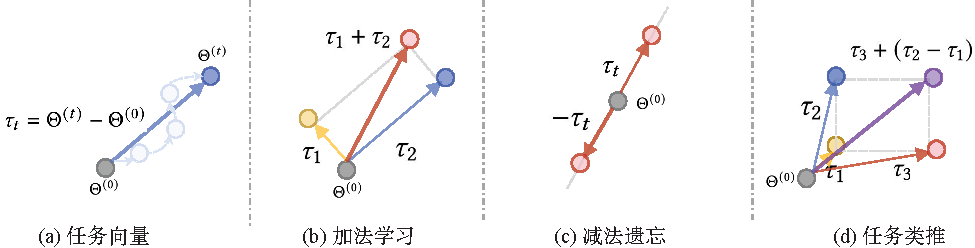
\includegraphics[width=\textwidth]{task-arithmetic-crop.pdf}
	\bicaption{任务算术\cite{editingmodelstask_ilharco_2023}的示意图。(a) “任务向量”的定义,即微调模型与预训练模型之间的差异。(b) 通过融合多个任务向量来实现多任务学习。(c) 通过减去任务向量来实现知识遗忘。(d) 使用类推任务向量来实现任务类推。}{An illustration of Task Arithmetic~\cite{editingmodelstask_ilharco_2023}. (a) Definition of the ``task vector'', which is the difference between the fine-tuned model and the pre-trained model. (b) Multi-task learning is performed by merging multiple task vectors. (c) Knowledge forgetting is achieved by subtracting the task vector. (d) Analogical task vectors are used to implement task analogies.}
	\label{fig:model-parameter-fusion}
\end{figure}
在此定义中,$\{\theta_i\}_{i=1}^n$ 代表 $n$ 个待融合模型的参数集合,这些参数通常是高维向量或张量。融合策略参数 $\alpha$ 则封装了具体的组合规则。$\alpha$ 的形式可以多种多样,例如它可以是一个简单的归一化权重向量 $\alpha = (\alpha_1, \dots, \alpha_n)$,用于计算参数的加权平均 $\theta_\mathrm{merged} = \sum_i \alpha_i \theta_i$;它也可以代表更复杂的、逐层或逐模块的融合权重;或者指示对参数(或参数增量)进行特定的选择、裁剪、对齐或算术运算(如任务算术中对 $\Delta \theta_i = \theta_i - \theta_{base}$ 的操作)。图~\ref{fig:model-parameter-fusion} 给出了任务算数的一个形象的描述。参数融合的优化问题,则是在给定的融合算子 $\text{Merge}$ 和允许的策略参数空间 $\mathcal{C}$(即 $\alpha \in \mathcal{C}$)下,寻找能够最大化融合模型在目标任务(或任务集) $\mathcal{T} = \{\tau_j\}$ 上综合性能 $F(\cdot, \mathcal{T})$ 的最优融合策略参数 $\alpha^*$:
\begin{equation}
	\alpha^* = \arg\max_{\alpha \in \mathcal{C}} F(\text{Merge}(\{\theta_i\}_{i=1}^n, \alpha), \mathcal{T}) \label{eq:merge_objective}
\end{equation}
其中 $F(\cdot, \mathcal{T})$ 是衡量模型在任务集 $\mathcal{T}$ 上综合表现的评估函数,例如多个任务性能指标(准确率、得分等)的加权平均。必须强调的是,此优化过程严格遵循免训练约束,即函数 $F$ 的评估仅依赖于对给定 $\alpha$ 生成的融合模型 $\theta_\mathrm{merged}(\alpha)$ 进行直接的推理评估,而不涉及任何训练数据的迭代或梯度计算。这使得参数融合在本质上成为一个高维、通常是黑盒的优化问题。

尽管参数融合的概念极具吸引力,但其在实践中面临的核心挑战在于稳定性差和性能难以保证的问题。简单或启发式的融合策略往往效果不佳,尤其是在融合的模型数量 $n$ 较大、模型来源(如微调数据、任务)差异显著(即异质性高)时。其根本原因在于深度神经网络参数空间的高度复杂性以及不同模型知识表示的潜在不兼容性——包括不同极小值之间的置换对称性与模式连通性等现象 \cite{gitrebasin_ainsworth_2023,losssurfacesmode_garipov_2018}。不同模型在各自的训练过程中可能收敛到损失函数景观的不同区域,即使它们在各自的任务上表现良好,其内部参数表示也可能存在语义上的错位或功能上的冲突。直接将这些参数进行组合,极易引发破坏性的干扰,导致融合模型的能力远低于各源模型的简单叠加,甚至出现灾难性的性能崩溃或能力遗忘。如何设计融合算子 $\text{Merge}$ 和优化策略 $\alpha$ 来智能地识别、量化、缓解或规避这些潜在的参数冲突,以确保融合过程的稳定性与有效性(即尽可能保留各源模型的优势能力),是该领域亟待解决的核心研究难点。

本文第 \ref{sec:ch5-knowledge-guided-multi-form-optimization-for-llm-fusion} 章的研究工作将重点聚焦于解决大规模、异质模型参数融合中的稳定性与效率这一核心科学问题。具体而言,研究将探索当待融合的模型数量 $n$ 较多,且这些模型代表了不同领域专长或经过不同任务微调(来源异质)时,如何设计一个有原则的、可扩展的免训练融合框架。该框架旨在通过引入显式的知识建模(如知识图谱)和更智能的优化策略(如多形式优化),在有效集成各模型能力的同时,最大限度地避免性能损失,并提升寻找高质量融合解的效率。这构成了第 \ref{sec:ch5-knowledge-guided-multi-form-optimization-for-llm-fusion} 章研究的核心问题背景与形式化设定。

\mysection{本章小结}
\label{sec:ch2-4-chapter-summary}

本章旨在为本文后续章节深入探讨深度模型高效构建的具体方法,奠定统一且必要的理论基础与预备知识。我们首先在 2.2 节中界定了贯穿全文的核心理念——知识迁移,阐明了其作为一种复用先验以提升效率的方法论思想,并剖析了该思想在本文所关注的知识、结构与参数三个研究维度中的不同体现形式与知识载体。随后,为了给后续的方法研究提供清晰的问题边界与目标,2.3 节分别对少样本学习与知识蒸馏、神经架构搜索与可迁移 NAS、以及参数融合这三个关键问题领域,给出了精炼的形式化定义。

通过对核心概念的界定、关键问题的形式化以及符号体系的统一,本章为理解本文后续提出的创新性方法提供了必要的理论支撑和共享语境。后续章节将正是在本章奠定的基础之上,展开对这些具体高效构建策略的详细阐述、算法设计与实验验证。

\end{document}
